\begin{figure}[htb]
  \centering
  \subfloat[$K_3$, planar]{
    \begin{tikzpicture}
      \fullyConnectedGraph{90,-30,180+30}{1cm}
    \end{tikzpicture}
  }
  \subfloat[$K_4$, planar]{
    \begin{tikzpicture}
      \fullyConnectedGraph{90-45, 90+45, -90-45, -90+45}{1cm}
    \end{tikzpicture}
  }
  \subfloat[$K_4$, planar, alternative]{
    \begin{tikzpicture}
      \fullyConnectedGraph{90,-30,180+30}{1cm}
      \node (n0) at (0,0) {};
      \fill (n0) circle(2pt);
      \foreach \i in {1,...,\the\value{nodecount}} {
	\path (n0) edge (n\i);
      };
    \end{tikzpicture}
  }
  \subfloat[$K_5$, nonplanar]{
    \begin{tikzpicture}
      \fullyConnectedGraph{90, 30, 180-30, -90-45, -90+45}{1.25cm}
    \end{tikzpicture}
  }
  \subfloat[$K_{3,3}$, nonplanar, bipartite]{
    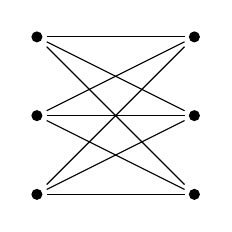
\begin{tikzpicture} % pipartite graph K_{3,3}
      \foreach \i in {1,...,3} {
	\node (n1\i) at (0,\i) {};
	\node (n2\i) at (2,\i) {};
	\fill (n1\i) circle(2pt);
	\fill (n2\i) circle(2pt);
      };
      \foreach \i in {1,...,3}
      {
	\foreach \j in {1,...,3}
	{
	  \path (n1\i) edge (n2\j);
	};
      };
    \end{tikzpicture}
  }
  \caption{Examples for (non-)planar Graphs}
\end{figure}

